\documentclass[11pt,letterpaper]{article}
\usepackage{fullpage}
\usepackage{multicol}
\usepackage{amsmath}
\usepackage{amsfonts}
\usepackage{amssymb}
%\usepackage{pstricks, pst-node, pst-plot}

\ifx\pdfoutput\undefined
% we are running LaTeX, not pdflatex
\usepackage{graphicx}
\else
% we are running pdflatex, so convert .eps files to .pdf
\usepackage[pdftex]{graphicx}
\usepackage{epstopdf}
\fi

\newcommand{\ds}{\displaystyle}
\newcommand{\bv}{\mathbf}
\newcommand{\lv}{\langle}
\newcommand{\rv}{\rangle}

\begin{document}
\flushleft
\begin{multicols}{2}


\begin{large}\textbf{Math 116 Quiz 4: Exam 1 Review \\
Tue 9 Oct 2012}\end{large}

\textbf{Name:  }\underline{\hspace{35ex}}

\vspace{.5in}

\end{multicols}

\pagestyle{empty}


\flushleft

You have 30 minutes to complete this quiz.  Eyes on your own paper and good luck!

\begin{enumerate}

\item \textbf{Definitions/Concepts.} -none this week-

\vspace{1pc}
\item \textbf{Questions/Problems.} 
\begin{enumerate}
\item {\it (Winter 2010 \# 7)} (7 pts) Given is a graph of $g'(x)$.  Sketch a graph of $g(x)$ on the provided axes, given that $g(0)=0$ and $g(x)$ is continuous.  On your graph, label all local maxima, minima, and points of inflection.
\smallskip
\begin{center}
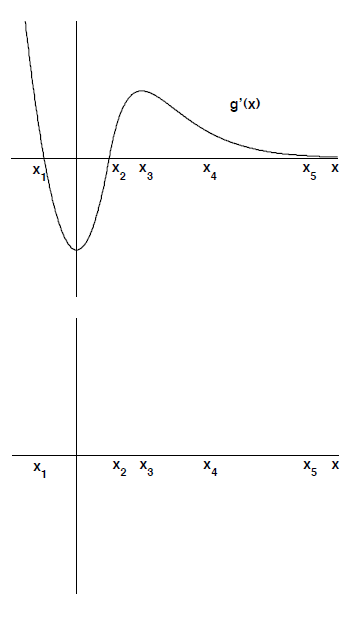
\includegraphics[width=.5\textwidth]{quiz4pic.png}
\end{center}

\vfill\hfill{\bf MORE QUIZ ON THE BACK --\textgreater}
\vfill
\item {\it (Winter 2011 \#7)}  A truck carrying a large tank of paint leaves a garage at 9 AM.  The tank starts to leak in such a way that $x$ miles from the garage, the density of paint on the road is $e^{-x^2/5000}$ gallons per mile.  At 10 AM, a cleaning crew leaves from the same garage and follows the path of the truck, scrubbing the paint from the road as it travels until it catches up to the leaking truck.  At $t$ hours after 10 AM, the leaking truck is $50\ln{(t+2)}$ miles from the garage, and the cleanup crew is $35t$ miles from the garage.  You may use your calculator to evaluate any definite integrals for this problem.

\smallskip
\begin{enumerate}
\item (4 pts) Calculate the total amount of paint that has leaked from the truck by 11 AM.

\vspace{10pc}
\item (3 pts) At time $t$ hours after 10 AM, what interval $I$ of the road is still covered in paint?  You may assume $t$ represents a time before the trucks meet.

\vspace{6pc}
\item (3 pts) Let $P(t)$ represent the amount of paint in gallons on the road $t$ hours after 10 AM.  Find a formula (which may include a definite integral) for $P(t)$.

\vspace{8pc}
\item (3 pts) Calculate $P'(1)$.

\vspace{8pc}
\end{enumerate}

\smallskip
%\item (Fall 2011 \#8) Let $f$ be a differentiable function with derivative $f'$.  A table of values for $f$ and $f'$ is given below.

%\smallskip
%\begin{center}
%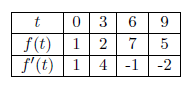
\includegraphics[width=.3\textwidth]{quiz4pic2.png}
%\end{center}

%\smallskip
%Find the exact value of the following integrals.

%\smallskip
%\begin{enumerate}
%\item (3 pts) $\int_0^1f'(3t)dt$

%\vspace{10pc}
%\item (5 pts) $\int_3^9tf''(t)dt$

%\vspace{10pc}
%\end{enumerate}

\end{enumerate}



\item \textbf{Computations/Algebra.} -none this week-

\end{enumerate}



\end{document}


